\documentclass[conference]{IEEEtran}
% Add the compsoc option for Computer Society conferences.
%
% If IEEEtran.cls has not been installed into the LaTeX system files,
% manually specify the path to it like:
% \documentclass[conference]{../sty/IEEEtran}
\usepackage[dvips]{epsfig}
\usepackage[english]{babel}
\usepackage[latin1]{inputenc}
\usepackage{mymacros}
\usepackage{booktabs}
%\usepackage[table]{xcolor}
\usepackage{multirow}
\usepackage{amssymb}
\usepackage{amsmath}
%\usepackage{url}
\usepackage{graphicx}
%\usepackage{graphics}
\usepackage{pstricks,pst-node,pst-tree}


\usepackage[caption=false,font=footnotesize]{subfig}
\usepackage{diagbox}


\usepackage{cite} % Loading the cite package will result in citation numbers being automatically sorted and properly "ranged". i.e., [1], [9], [2], [7], [5], [6] (without using cite.sty) will become: [1], [2], [5]--[7], [9] (using cite.sty)
\usepackage{stfloats}  % Gives LaTeX2e the ability to do double column
                        % floats at the bottom of the page as well as the top.
                        % (e.g., "\begin{figure*}[!b]" is not normally
                        % possible in LaTeX2e). This is an invasive package
                        % which rewrites many portions of the LaTeX2e output
                        % routines. It may not work with other packages that
                        % modify the LaTeX2e output routine and/or with other
                        % versions of LaTeX.

% correct bad hyphenation here
%\hyphenation{op-tical net-works semi-conduc-tor IEEEtran}



% *** GRAPHICS RELATED PACKAGES ***
%
\ifCLASSINFOpdf
  % \usepackage[pdftex]{graphicx}
  % declare the path(s) where your graphic files are
  % \graphicspath{{../pdf/}{../jpeg/}}
  % and their extensions so you won't have to specify these with
  % every instance of \includegraphics
  % \DeclareGraphicsExtensions{.pdf,.jpeg,.png}
\else
  % or other class option (dvipsone, dvipdf, if not using dvips). graphicx
  % will default to the driver specified in the system graphics.cfg if no
  % driver is specified.
  % \usepackage[dvips]{graphicx}
  % declare the path(s) where your graphic files are
  % \graphicspath{{../eps/}}
  % and their extensions so you won't have to specify these with
  % every instance of \includegraphics
  % \DeclareGraphicsExtensions{.eps}
\fi
% graphicx was written by David Carlisle and Sebastian Rahtz. It is
% required if you want graphics, photos, etc. graphicx.sty is already
% installed on most LaTeX systems. The latest version and documentation can
% be obtained at: 
% http://www.ctan.org/tex-archive/macros/latex/required/graphics/
% Another good source of documentation is "Using Imported Graphics in
% LaTeX2e" by Keith Reckdahl which can be found as epslatex.ps or
% epslatex.pdf at: http://www.ctan.org/tex-archive/info/
%
% latex, and pdflatex in dvi mode, support graphics in encapsulated
% postscript (.eps) format. pdflatex in pdf mode supports graphics
% in .pdf, .jpeg, .png and .mps (metapost) formats. Users should ensure
% that all non-photo figures use a vector format (.eps, .pdf, .mps) and
% not a bitmapped formats (.jpeg, .png). IEEE frowns on bitmapped formats
% which can result in "jaggedy"/blurry rendering of lines and letters as
% well as large increases in file sizes.
%
% You can find documentation about the pdfTeX application at:
% http://www.tug.org/applications/pdftex





% *** MATH PACKAGES ***
%
%\usepackage[cmex10]{amsmath}
% A popular package from the American Mathematical Society that provides
% many useful and powerful commands for dealing with mathematics. If using
% it, be sure to load this package with the cmex10 option to ensure that
% only type 1 fonts will utilized at all point sizes. Without this option,
% it is possible that some math symbols, particularly those within
% footnotes, will be rendered in bitmap form which will result in a
% document that can not be IEEE Xplore compliant!
%
% Also, note that the amsmath package sets \interdisplaylinepenalty to 10000
% thus preventing page breaks from occurring within multiline equations. Use:
%\interdisplaylinepenalty=2500
% after loading amsmath to restore such page breaks as IEEEtran.cls normally
% does. amsmath.sty is already installed on most LaTeX systems. The latest
% version and documentation can be obtained at:
% http://www.ctan.org/tex-archive/macros/latex/required/amslatex/math/





% *** SPECIALIZED LIST PACKAGES ***
%
%\usepackage{algorithmic}
% algorithmic.sty was written by Peter Williams and Rogerio Brito.
% This package provides an algorithmic environment fo describing algorithms.
% You can use the algorithmic environment in-text or within a figure
% environment to provide for a floating algorithm. Do NOT use the algorithm
% floating environment provided by algorithm.sty (by the same authors) or
% algorithm2e.sty (by Christophe Fiorio) as IEEE does not use dedicated
% algorithm float types and packages that provide these will not provide
% correct IEEE style captions. The latest version and documentation of
% algorithmic.sty can be obtained at:
% http://www.ctan.org/tex-archive/macros/latex/contrib/algorithms/
% There is also a support site at:
% http://algorithms.berlios.de/index.html
% Also of interest may be the (relatively newer and more customizable)
% algorithmicx.sty package by Szasz Janos:
% http://www.ctan.org/tex-archive/macros/latex/contrib/algorithmicx/




% *** ALIGNMENT PACKAGES ***
%
%\usepackage{array}
% Frank Mittelbach's and David Carlisle's array.sty patches and improves
% the standard LaTeX2e array and tabular environments to provide better
% appearance and additional user controls. As the default LaTeX2e table
% generation code is lacking to the point of almost being broken with
% respect to the quality of the end results, all users are strongly
% advised to use an enhanced (at the very least that provided by array.sty)
% set of table tools. array.sty is already installed on most systems. The
% latest version and documentation can be obtained at:
% http://www.ctan.org/tex-archive/macros/latex/required/tools/


%\usepackage{mdwmath}
%\usepackage{mdwtab}
% Also highly recommended is Mark Wooding's extremely powerful MDW tools,
% especially mdwmath.sty and mdwtab.sty which are used to format equations
% and tables, respectively. The MDWtools set is already installed on most
% LaTeX systems. The lastest version and documentation is available at:
% http://www.ctan.org/tex-archive/macros/latex/contrib/mdwtools/


% IEEEtran contains the IEEEeqnarray family of commands that can be used to
% generate multiline equations as well as matrices, tables, etc., of high
% quality.


%\usepackage{eqparbox}
% Also of notable interest is Scott Pakin's eqparbox package for creating
% (automatically sized) equal width boxes - aka "natural width parboxes".
% Available at:
% http://www.ctan.org/tex-archive/macros/latex/contrib/eqparbox/





% *** SUBFIGURE PACKAGES ***
%\usepackage[tight,footnotesize]{subfigure}
% subfigure.sty was written by Steven Douglas Cochran. This package makes it
% easy to put subfigures in your figures. e.g., "Figure 1a and 1b". For IEEE
% work, it is a good idea to load it with the tight package option to reduce
% the amount of white space around the subfigures. subfigure.sty is already
% installed on most LaTeX systems. The latest version and documentation can
% be obtained at:
% http://www.ctan.org/tex-archive/obsolete/macros/latex/contrib/subfigure/
% subfigure.sty has been superceeded by subfig.sty.



%\usepackage[caption=false]{caption}
%\usepackage[font=footnotesize]{subfig}
% subfig.sty, also written by Steven Douglas Cochran, is the modern
% replacement for subfigure.sty. However, subfig.sty requires and
% automatically loads Axel Sommerfeldt's caption.sty which will override
% IEEEtran.cls handling of captions and this will result in nonIEEE style
% figure/table captions. To prevent this problem, be sure and preload
% caption.sty with its "caption=false" package option. This is will preserve
% IEEEtran.cls handing of captions. Version 1.3 (2005/06/28) and later 
% (recommended due to many improvements over 1.2) of subfig.sty supports
% the caption=false option directly:
%\usepackage[caption=false,font=footnotesize]{subfig}
%
% The latest version and documentation can be obtained at:
% http://www.ctan.org/tex-archive/macros/latex/contrib/subfig/
% The latest version and documentation of caption.sty can be obtained at:
% http://www.ctan.org/tex-archive/macros/latex/contrib/caption/




% *** FLOAT PACKAGES ***
%
%\usepackage{fixltx2e}
% fixltx2e, the successor to the earlier fix2col.sty, was written by
% Frank Mittelbach and David Carlisle. This package corrects a few problems
% in the LaTeX2e kernel, the most notable of which is that in current
% LaTeX2e releases, the ordering of single and double column floats is not
% guaranteed to be preserved. Thus, an unpatched LaTeX2e can allow a
% single column figure to be placed prior to an earlier double column
% figure. The latest version and documentation can be found at:
% http://www.ctan.org/tex-archive/macros/latex/base/



%\usepackage{stfloats}
% stfloats.sty was written by Sigitas Tolusis. This package gives LaTeX2e
% the ability to do double column floats at the bottom of the page as well
% as the top. (e.g., "\begin{figure*}[!b]" is not normally possible in
% LaTeX2e). It also provides a command:
%\fnbelowfloat
% to enable the placement of footnotes below bottom floats (the standard
% LaTeX2e kernel puts them above bottom floats). This is an invasive package
% which rewrites many portions of the LaTeX2e float routines. It may not work
% with other packages that modify the LaTeX2e float routines. The latest
% version and documentation can be obtained at:
% http://www.ctan.org/tex-archive/macros/latex/contrib/sttools/
% Documentation is contained in the stfloats.sty comments as well as in the
% presfull.pdf file. Do not use the stfloats baselinefloat ability as IEEE
% does not allow \baselineskip to stretch. Authors submitting work to the
% IEEE should note that IEEE rarely uses double column equations and
% that authors should try to avoid such use. Do not be tempted to use the
% cuted.sty or midfloat.sty packages (also by Sigitas Tolusis) as IEEE does
% not format its papers in such ways.





% *** PDF, URL AND HYPERLINK PACKAGES ***
%
%\usepackage{url}
% url.sty was written by Donald Arseneau. It provides better support for
% handling and breaking URLs. url.sty is already installed on most LaTeX
% systems. The latest version can be obtained at:
% http://www.ctan.org/tex-archive/macros/latex/contrib/misc/
% Read the url.sty source comments for usage information. Basically,
% \url{my_url_here}.





% *** Do not adjust lengths that control margins, column widths, etc. ***
% *** Do not use packages that alter fonts (such as pslatex).         ***
% There should be no need to do such things with IEEEtran.cls V1.6 and later.
% (Unless specifically asked to do so by the journal or conference you plan
% to submit to, of course. )




\begin{document}
%
% paper title
% can use linebreaks \\ within to get better formatting as desired
\title{Scenario-based Reasoning through Dynamic Decision Networks for Countering Maritime Drug Trafficking} % choose your own 

% author names and affiliations
% use a multiple column layout for up to three different
% affiliations
\author{\IEEEauthorblockN{Patrick de Oude}  
\IEEEauthorblockA{D-CIS Lab\\
Thales Research and Technology\\
Delft, The Netherlands\\
Email: patrick.deoude@d-cis.nl}
\and
\IEEEauthorblockN{Tom Pepels}
\IEEEauthorblockA{D-CIS Lab\\
Thales Research and Technology\\
Delft, The Netherlands\\
Email: tom.pepels@d-cis.nl}
\and
\IEEEauthorblockN{Rik Claessens}
\IEEEauthorblockA{D-CIS Lab\\
Thales Research and Technology\\
Delft, The Netherlands\\
Email: rik.claessens@d-cis.nl}
}

% make the title area
\maketitle


\begin{abstract}
The abstract comes here.
\end{abstract}
% IEEEtran.cls defaults to using nonbold math in the Abstract.
% This preserves the distinction between vectors and scalars. However,
% if the conference you are submitting to favors bold math in the abstract,
% then you can use LaTeX's standard command \boldmath at the very start
% of the abstract to achieve this. Many IEEE journals/conferences frown on
% math in the abstract anyway.

% no keywords



% For peer review papers, you can put extra information on the cover
% page as needed:
% \ifCLASSOPTIONpeerreview
% \begin{center} \bfseries EDICS Category: 3-BBND \end{center}
% \fi
%
% For peerreview papers, this IEEEtran command inserts a page break and
% creates the second title. It will be ignored for other modes.
\IEEEpeerreviewmaketitle

%%% Comment out itemize environments when writing your section

\section{Introduction}

% \begin{itemize}
% \item Introduce and describe the problem (what + why)
% \item introduce the MH370 scenario
% \end{itemize}


Decision making in contemporary complex domains, such as large-scale crisis management, Search \& Rescue operations, border security, anti-drug operations etc., can pose an enormous cognitive challenge on the decision maker. Decision makers often need to construct and manage multiple {\em scenarios} regarding the situation description in order to deal with uncertainties that are encountered in these domains. A scenario is a projected or imagined sequence of events describing what could possibly happen (or have happened). By keeping track of the possible scenarios that are compatible with the known information the decision maker can maintain multiple states of situation awareness that are required to be able to make the right decision at the right moment in time. However, the set of possible scenarios may become significantly large in complex real-world applications (typically involving numerous factors and uncertainties), while human cognitive limitations pose restrictions on the number of scenarios that decision makers can effectively handle at any given time. Therefore, to be able to effectively manage a (possibly large) set of scenarios, and to ultimately decide on the information to be presented to the decision makers, automated managing of scenarios must be addressed.

A scenario can be considered a narration concerning various events that have materialized (or going to materialize) over time. These events are often causally dependent on each other and can be captured as variables in a causal model \cite{pearl00book}. In \cite{conrado14if} we have shown that these causal models support {\em scoping of states} of scenario variables. Moreover, such causal models can be captured through Bayesian networks (BNs) \cite{pearl88book, jensen07book} to provide a convenient framework to manage a large set of scenarios through: (i) pruning of insignificant scenarios, (ii) updating the scenarios based on new observations and (iii) computing the likelihood of a scenario given the latest information to establish an ordering on the set of relevant scenarios. Additionally, BNs allows what-if exploration where, for example, the likelihood of certain (future) events are computed based on various assumptions about the occurrence of other events of the scenario.

While BNs provide an effective way to manage scenarios it does not allow the actual decisions taken by the decision maker to be modeled. Neither do they provide advise on which decision the decision maker should take. In this paper the model is extended by describing the structure of the decision process as well. This allows the model to give advice about the actual decisions the decision maker wants to consider. The extended model is called a {\em decision network} \cite{russell02bn} (also influence diagram or decision graph \cite{jensen07book}) and includes next to the chance nodes also decision and utility nodes. Influence diagrams also supports assessment of risk by, for example, computing the worst case scenario\footnote{The worst-case scenario is not necessarily the most likely scenario} considering the utilities in the model.



% In \cite{conrado14if} a method was discussed to manage the set of possible scenarios using Bayesian networks (BNs) \cite{pearl88book, jensen07book}. With the help of BN an estimate of the likelihood of the scenario to unfold can be computed given the evidence that is available at the time. With these likelihoods the set of scenarios can be ranked form most to least likely scenario, which enables the decision maker to focus on the set of most likely scenarios. The method described there did not model the actual decisions that a decision maker could make. In this paper 



%


%TODO add related work about the use of influence diagrams and secenario based reasoning

% In the BNIn this paper we are going to extend the framework discussed in \cite{conrado14if} with the actual decision
% 
% 
% The models consist only of chance nodes which do not support assessment of risk since this would require utilities to be part of the model. For example, to compute the worst case scenario, which is not necessarily the most likely, information is required about the impact of the scenario. To support risk assessment the framework discussed in \cite{conrado14if} is extended with decision and utility nodes.
% 
% 
% 
% t When time progresses, new evidence might be obtained and the likelihood of the scenarios can be updated.




% When making decisions in complex contemporary applications, e.g. intelligence operations and large-scale crisis management, decision makers often need to construct and manage multiple hypotheses regarding the situation description in order to deal with uncertainties. Hypotheses about a situation's description are commonly referred to as {\em scenarios}. A scenario can be defined as a projected or imagined sequence of events describing what could possibly happen (or have happened). Scenarios can be used to deal with uncertainty by allowing the exploration of diverse descriptions of a given situation (and its possible developments) that are compatible with known information at any given time. Scenarios can thus offer multiple states of situation awareness and help overcome cognitive biases, and as such should ideally explore the whole set of plausible and relevant states of the world. Owing to human cognitive limitations, however, keeping track of all relevant information can become a challenge, even when only a few scenarios are considered.


%TODO add overview of the paper





\section{Causal Models}

%TODO explain the scenario

Maritime drug trafficking is an ongoing problem in the Caribbean sea. Very fast and small vessels, so called go-fasts, are used to transport contraband from Columbia's and Venezuela's coast to Jamaica, Haiti and Dominican Republic to be further transported into North-America. The popularity of a go-fast to be used as a drug trafficking vehicle is due to the go-fast's size, speed and low radar and optical signatures. This makes go-fasts hard to detect and difficult to intercept by often slower coast guard vehicles. Nevertheless, the U.S. coast guard deploys their own go-fasts and helicopters equipped with anti-materiel rifles (AMR) to disable the engine of a running go-fast. 

The main challenge of anti-drug trafficking organizations, such as the coast guard, is to locate the smuggler's go-fast in order to intercept it. There are several type of observations that can be used. Location of the smuggler's go-fast can be determined by radar ($RO$) in case of calm sea or at close range or by visual observation ($VO$). A more recent type of observation is through the use of sonar mounted on buoys in the ocean ($SO$) that can register the typical engine sound of go-fast. Unfortunately, these type of observation might not be available. For radar and sonar the coverage is often limited and, therefore, not always available. Visual observations is only possible if an observer is close enough to report about it. With the knowledge of the location of the smuggler's go-fast allows us the reason about the possible intercept areas. This area can be a location where the smuggler's go-fast currently is or a more strategic position that is believed to be visited by the smugglers at some point in the future. These strategic positions are inferred from Intel collected during the anti-drug operations, for example. There might be Intel that the smugglers need to refuel at some refueling location along their route ($RA$). This belief is based on Intel about the amount of fuel loaded on board prior to departure ($AF$), the possible destination ($D$) and the possible locations where refueling is possible ($LR$). If there is strong belief that the smugglers are going to refuel at a certain location then that location is a possible intercept area. In Figure~\ref{fig:causal-model} the causal model is depicted that describes the causal influences between these variables. All the variables are listed in Table~\ref{tab:scenario-variables}.


\begin{figure}
\begin{center}
 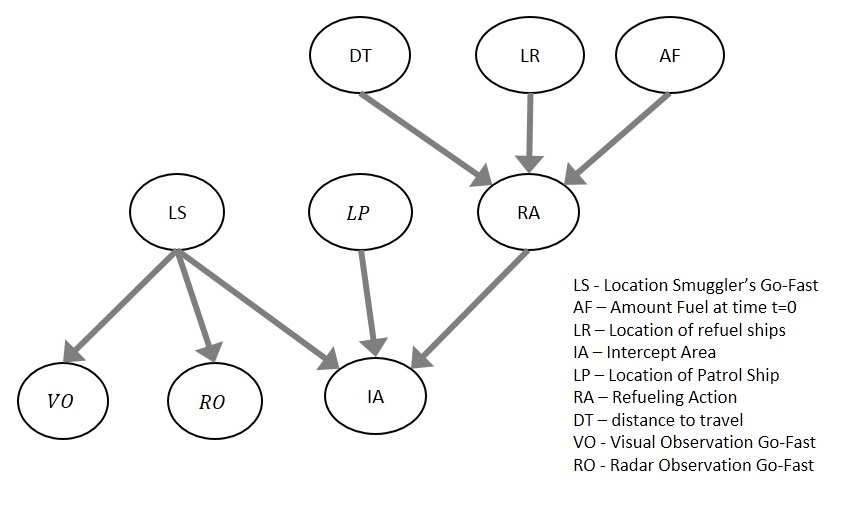
\includegraphics[width=.4\textwidth]{causal-model.eps}
 \caption{Causal model of the smuggler scenario}\label{fig:causal-model}
 % decision-graph.eps: 0x0 pixel, 300dpi, 0.00x0.00 cm, bb=-0 -0 424 277
\end{center}
\end{figure}


\begin{table}[!ht]
 \centering
 \caption{Overview of scenario variables from the causal model shown Figure~\ref{fig:causal-model}, as well as their semantics.}
 \begin{tabular}[!ht]{rp{5cm}}
\toprule
 Variable & Semantics \\
\cmidrule(r){1-1}
\cmidrule(l){2-2}
$LocationSmuggler$ ($LS$) &
The location of the smuggler's go-fast. \\
$Destination$ ($D$) &
Destination to which the smugglers travel. \\
$LocationRefuel$ ($LR$) &
Locations of stationary refuel ships in the concerned area of the sea. \\
$Weather$ ($W$) &
Weather conditions (for the concerned area and time) relevant for the smugglers' traveling. \\
$RefuelingAction$ ($RA$) &
Occurrence (or not) of a refueling action by the smugglers, as well as its position. \\
$InterceptVehicle$ ($IV$) &
Location of an available intercept vehicle. This could either be coast guard's go-fast or helicopter etc. \\
$InterceptArea$ ($IA$) &
Area where the intercept vehicles can intercept the smugglers' go-fast. \\
\bottomrule
\end{tabular}
%\caption{Overview of scenario variables from the causal graphs in Figure~\ref{fig:causal-graph1} and \ref{fig:causal-graph2}, as well as their semantics.}\label{tab:cpt-example}
\label{tab:scenario-variables}
\end{table}


% Timely response in Search and Rescue (SAR) operations is most critical in the first few hours after the emergency has taken place. Generally after the initial hours of the incident the chances of finding possible survivors is significantly reduced. Before the actual rescue operation can commence the main challenge is to locate the incident site. In order to locate the incident site the available resources, such as helicopter, planes, ships, search crew, dogs, etc. must deployed as fast as possible at the right location to minimize the localization time. In order to determine initial search location observation that can be used to infer the the possible incident location can be used.


\section{Decision Network}\label{sec:influence-diagrams}

In \cite{conrado14if} we used BNs to represent a symmetric scenario tree capturing all possible scenarios given the modeled scenario variables. The decision maker can use this BN to manage the set of scenario using probabilistic inference to do pruning, ranking and what-if exploration. Based on this information the decision maker decides on which course of action is best by making a decision. This decision results in an action or a set of actions that influences further development of the scenario. For example, sailing my intercept vehicle in the wrong direction moving away from the smugglers results in fewer or none possible intercept areas. In this paper we extend the scenario reasoning framework discussed in \cite{conrado14if} to include the decision maker's decisions explicitly. The models that allows us to model decisions into the BN are called decision network. A {\em decision network (DN)} (also influence diagram or decision graph \cite{russell02bn,howard84rpada,jensen07book}) is a concise graphical and mathematical representation of a decision problem. DNs are a generalization of BNs so we therefore start discussing BNs first.


\begin{figure}
\begin{center}
 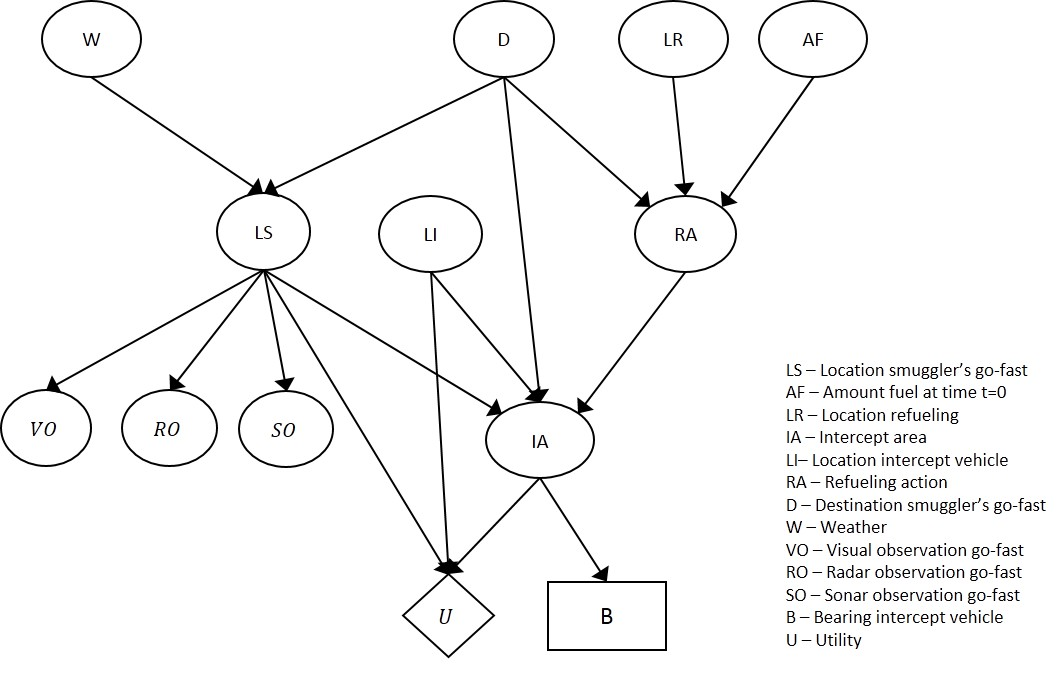
\includegraphics[width=.4\textwidth]{decision-network.eps}
 \caption{Decision network based on the causal model shown in Figure~\ref{fig:causal-model}.\label{fig:decision-graph}}
 % decision-graph.eps: 0x0 pixel, 300dpi, 0.00x0.00 cm, bb=-0 -0 424 277
\end{center}
\end{figure}


\subsection{Bayesian networks}\label{sec:bayesian-networks}

% \begin{figure}
%  \centering
% \subfloat[\label{fig:bn-example}]{\scalebox{.7}{
% $
% \psmatrix[colsep=.7cm,rowsep=.7cm,mnode=circle]
%  & [name=W] W  \\
% [name=D] D & & [name=I] I\; \\
%  & [name=A] A \\
% [name=F] F 
% \psset{arrowscale=2}
% \psset{nodesep=1pt}
% \ncline{->}{W}{I}
% \ncline{->}{D}{I}
% \ncline{->}{D}{A}
% \ncline{->}{F}{A}
% \ncline{->}{A}{I}
% \endpsmatrix$}}\qquad
% \subfloat[\label{fig:bn-example2}]{\scalebox{.7}{
% $
% \psmatrix[colsep=.7cm,rowsep=.7cm,mnode=circle]
%  & [name=W] W  \\
% [name=D] D & & [name=I] I\; \\
%  & [name=A] A \\
% [name=F] F & & [name=R] R
% \psset{arrowscale=2}
% \psset{nodesep=1pt}
% \ncline{->}{W}{I}
% \ncline{->}{D}{I}
% \ncline{->}{D}{A}
% \ncline{->}{F}{A}
% \ncline{->}{A}{I}
% \ncline{->}{A}{R}
% \endpsmatrix$}}\\[10pt]
% \subfloat[\label{fig:cpt-example}]{
%  \begin{tabular}{r|ccc|c|c} 
% $D$	& \multicolumn{3}{c|}{X} & Y &  Z \\ 
%  \diagbox{$A$}{$F$} & Small & Medium & Large & & \\
% \hline
%  No & 0.1 & 1 & 1 & \ldots & \ldots \\
%  Yes at 1 & 0.9 & 0 & 0 & \ldots & \ldots \\ 
%  Yes at 2 & 0 & 0 & 0 & \ldots & \ldots \\ 
%  Yes at 3 & 0 & 0 & 0 & \ldots & \ldots \\ 
%  \end{tabular}}
% \caption{Bayesian network of the causal model shown in Figure~\ref{fig:causal-graph1} (a) and Figure~\ref{fig:causal-graph2} (b), as well as a CPT of the discrete conditional probability distribution $P(A|D,F)$ (c).}
% \end{figure}

{\red needs to be reworked - Patrick}


A Bayesian network (BN) is a probabilistic graphical model that efficiently represents a joint probability distribution (JPD) over a set of random variables \cite{jensen01book,pearl88book}. A BN is represented through a Directed Acyclic Graph (DAG), where each node in the DAG corresponds to a random variable of the JPD. For example, the causal graphs shown in Figure~ 2 can be captured by the DAGs shown in Figure 5a and~\ref{fig:bn-example}, where scenario variables (solid circles in Figure 2) are represented as random variables (nodes), and each possible scenario variable state corresponds to a random variable state. 
Note that, the range of states for the scenario variables (and therefore the range of states for the random variables) is not determined a priori but as the estimation processes take place, as explained in section II, on scoping of states.
For each node given its parents in the DAG, a conditional probability distribution (CPD) needs to be specified. For instance, the CPD $P(A|D,F)$ must be specified for the variable $RefuelingAction$ ($A$). Discrete CPDs can be represented through conditional probability tables (CPTs).  Since the variables $D$, $F$ and $A$ are discrete, the CPD $P(A|D,F)$ can be represented through the CPT shown in Figure~\ref{fig:cpt-example}. This CPT expresses that, given destination X and a small amount of fuel on board, the chance that a refueling action takes place (at location 1) is $0.9$, i.e. $P$($A$~=~Yes~at~1$|$$D$~=~X,~$F$~=~Small) = 0.9. For larger amounts of fuel (and the same destination X), it is estimated that no refueling action takes place. Moreover, there is no chance that the refueling action takes place at locations 2 and 3, as these locations are farther than X itself. This example shows that incompatibility of state combinations can simplify the specification of CPTs for scenario variables, as the probabilities of such combinations are zero.

Before the introduction of BNs, probabilistic inferences were performed directly on a JPD defined over several variables. This, however, limited such operations only to JPDs defined over a small set of variables due to the combinatorial complexity. A Bayesian network, on the other hand, exploits conditional independencies between the random variables. Consequently, the JPD can be factorized into CPDs for each variable in the model. 
For example, considering the BN shown in Figure 5a, the JPD $P(\VV)$ (where $\VV$\footnote{In this section, a single random variable is presented as an uppercase letter and its states as lowercase letters. A set of random variables and of states are shown as bold uppercase and bold lowercase letters, respectively.} = $\{W, D, F, A, I\}$) factorizes into a set of CPDs, i.e.


\begin{eqnarray}
P(\VV) = \prod_i P(X_i|\Pa(X_i)),  \label{eq:chain-rule}
\end{eqnarray}

\noindent
where $\Pa(X_i)$ denotes the parents of node $X_i$. For the BN in Figure 5a, the JPD is therefore

\begin{eqnarray}
 P(W,D,F,A,I) &=& P(W)P(D)P(F)P(A|D,F) \nonumber \\
  & & \cdot P(I|W,D,A). \nonumber
\end{eqnarray}


With the help of the chain rule in Equation~(\ref{eq:chain-rule}), a JPD can be represented through its factorization of CPDs, which requires significant fewer parameters compared to the number of parameters in the JPD. Moreover, by exploiting the conditional independencies between the random variables, efficient exact inference methods can be used, e.g. the junction tree algorithm \cite{cowell99bn}.

The likelihood of scenarios can be computed with the help of Equation~(\ref{eq:chain-rule}), given a BN of the causal model that shows the cause-effect relations between the scenario variables. For instance, for the scenario corresponding to the uppermost complete branch of the scenario tree in Figure~\ref{fig:scenario-tree}, i.e. $W$~=~bad, $D$~=~X, $F$~=~Small, $A$~=~Yes at 1, $I$~=~4, the likelihood can be computed as

\begin{eqnarray}
 P(W=\text{bad}, D=\text{X}, F=\text{Small}, A=\text{Yes at 1}, I=\text{4}) &=& \nonumber \\
 P(W=\text{bad})P(D=\text{X})P(F=\text{Small}) & & \nonumber \\ 
 \cdot P(A=\text{Yes at 1}|D=\text{X},F=\text{Small}) \nonumber \\
 \cdot P(I=\text{4}|W=\text{bad},D=\text{X},A=\text{Yes at 1}). \nonumber
\end{eqnarray}

  
Moreover, one of the main strengths of BNs is the possibility to perform predictive or diagnostic inference based on a given set of evidence denoted by $\E$. For example, in the second phase of the example the weather is observed, i.e. $\E = \{W = \text{bad}\}$. With this observation, the likelihood of the scenarios can be updated by computing $P(\vv|\E)$, where $\vv$ is a configuration of random variables states corresponding to a given scenario. Note that all scenarios with $W = \text{good}$ will get zero probability due to the observation. Assigning zero probabilities to scenarios after an observation update corresponds to pruning of scenarios based on evidence.

Also in the second phase of the example (whose BN is shown in Figure~\ref{fig:bn-example}), a new variable $R$ is added to the model to capture the received refuel report. The model needs to be updated by specifying the CPD $P(R|A)$ as well. The new JPD $P(W,D,F,A,I,R) = P(W)P(D)P(F)P(A|D,F)P(I|W,D,A)P(R|A)$ can be used to re-compute the likelihood of the scenarios, given the occurrence of the refueling report at position 1.


\begin{figure*}[!t]
\begin{center}
 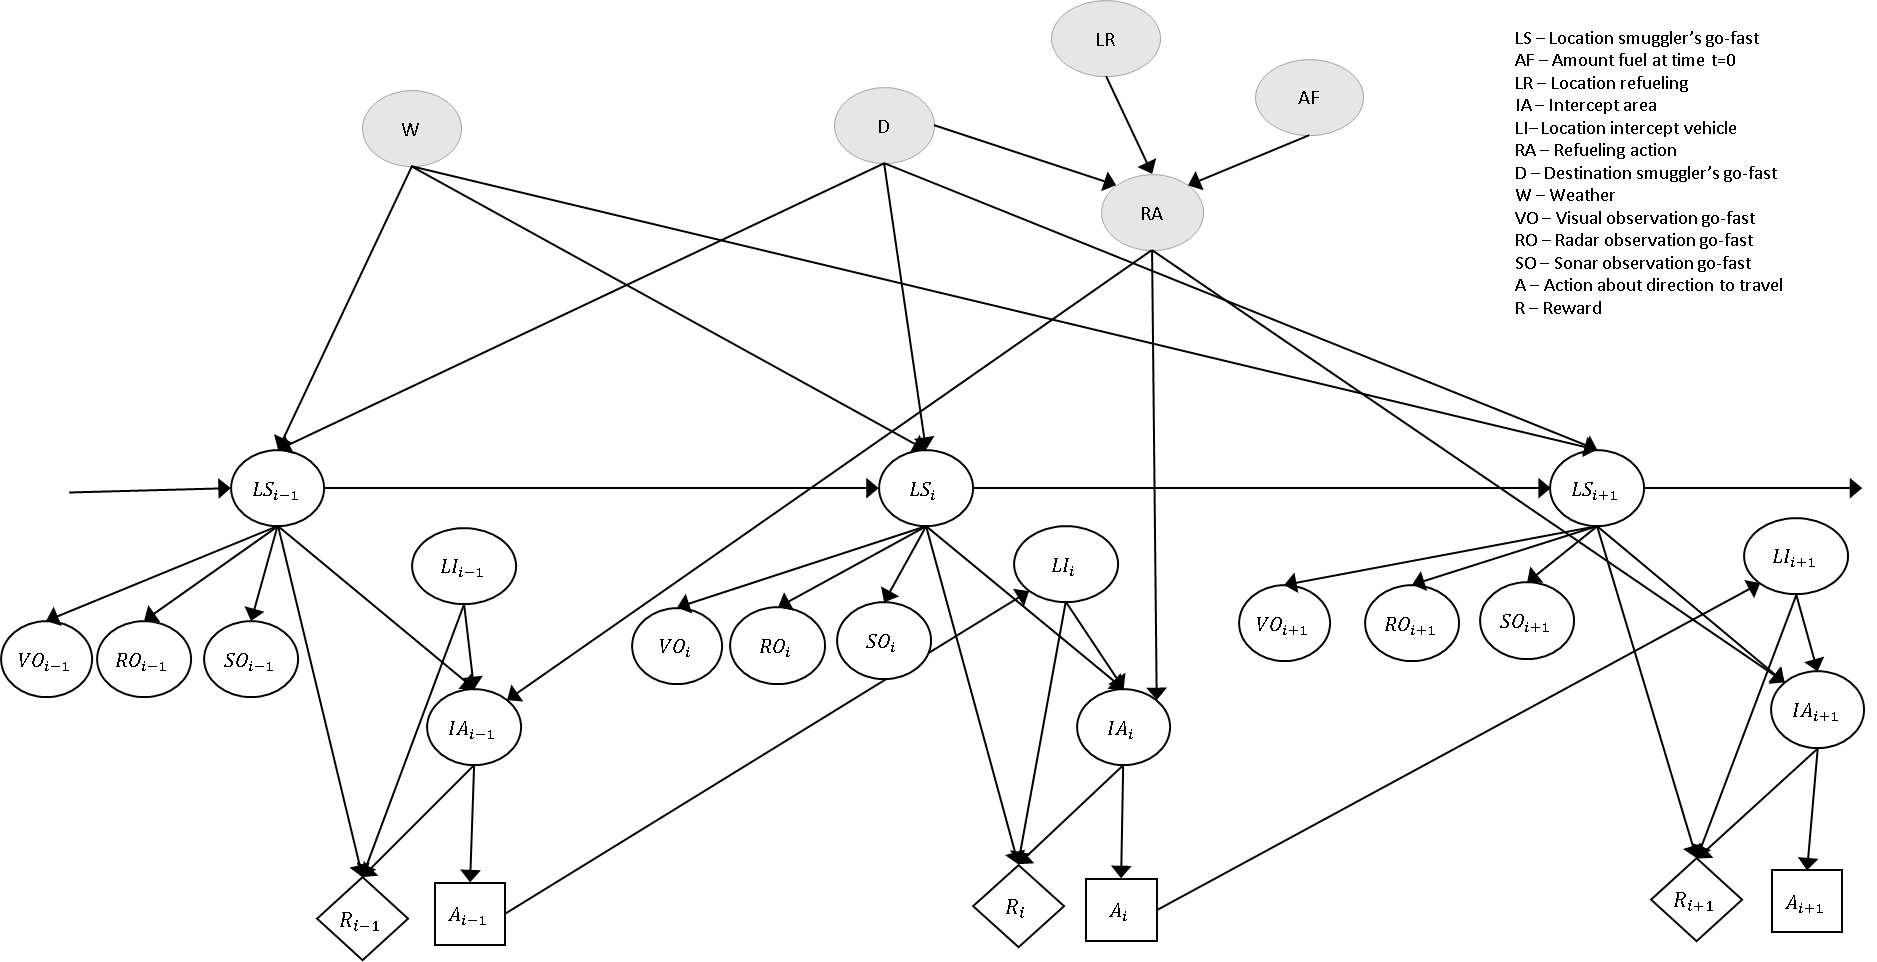
\includegraphics[width=.95\textwidth]{dynamic-decision-graph.eps}
 \caption{Dynamic decision graph of the influence diagram shown in Figure~\ref{fig:decision-graph}.}
 % decision-graph.eps: 0x0 pixel, 300dpi, 0.00x0.00 cm, bb=-0 -0 424 277
\end{center}
\end{figure*}


\subsection{Decision network}

{\red needs to be reworked - Patrick}




The BN described in the previous section can be extended into the decision network (DN) shown in Figure~\ref{fig:decision-graph}. This DN consists of the same nodes as in the causal model in Figure~\ref{fig:causal-model} plus a decision node $D$ and a utility node $U$. A decision node represents possible actions the decision maker can take. In this case the actions are the different directions the patrol ship can travel, such as North, East, South-west, etc. The utility node, on the other hand, represents the utility function where the parents of the utility node, i.e. $\{LS,LP,IA\}$, are the arguments of this function:

\[
 U(LS,LP,IA) = -\alpha d(LS,LP) - (1-\alpha) d(IA,LP),
\]

where $d(X,Y)$ is the distance between $X$ and $Y$ and $\alpha$ is a value between $[0,1]$ that is used to control the importance of either $d(LS,LP)$ or $d(IA,LP)$. In case $\alpha=1$ the utility function is $U(LS,LP,IA) = -d(LS,LP)$ and therefore solely based on the distance between the smuggler's boat and the patrol ship, while $\alpha=0$ the utility function is solely based on the distance of the patrol ship and the intercept area. The choice of $\alpha$ should be based on the information that is available. If more information is available that could help to locate the smuggler's go-fast then we want to weight  $d(LS,LP)$ more by using a higher $\alpha$ value. A higher utility is obtained when the patrol ship is either closer to the smuggler's location or to an intercept area (where eventually the smugglers should travel to).


% In order to evaluate the different decisions modeled in a DN the impact of the decision's consequences need to be measured. The consequence of a decision is measured through a utility node. For example, we need to drive to work either via route A or route B in the shortest amount of time. Clearly in this case the utility is based on the amount of time required to travel to work and the route that results in the lowest amount of time gets a higher associated utility value. In Figure~\ref{fig:decision-graph} an example of a DN is shown with a single decision variable (square node) and utility variable (diamond node) together with several random variables (oval nodes). Since a DN is generalization of a BN we start discussing BNs first.


\subsection{Dynamic Decision Networks}

{\red Explain the basics of DDN - Patrick}
In the Figure~\ref{fig:decision-graph} a static influence diagram was shown. However, intercepting a smuggler's go-fast is very dynamic environment where the location of the go-fast and the patrol ship are constantly changing. In these environment sequential decision making is required in order to successfully intercept the go-fast. In Figure~\ref{fig:dynamic-decision-graph} a {\em dynamic decision network (DDN)} is shown based on the influence diagram shown in Figure~\ref{fig:decision-graph}. The DDG \ldots

\subsection{Partially Observable Markov Decision Process}

{\red Explain definition of POMDP as a seq. decis. making proc. - Tom}
{\red Also extend to multi-agent POMDP, reduceability}

% Making decisions based on a POMDP defined in the previous section

\section{Scenario-Based Decision-Making}

\subsection{Planning Under Uncertainty}

{\red Method to find decisions based on repeated sampling of the state-space. requires: Discrete action model and state space, and a method of defining the current belief of the smuggler's location. - Tom}

\subsection{State Representation}

{\red How do we represent the possible states - Tom}

\subsection{State Estimation}

{\red how do we estimate the position of the smugglers based on the observations: use of particle filter + scenario context - Rik}

\subsection{Multi-Agent Decision Making}

{\red some thoughts on how to handle these kind of problems (i.e. MPOMDP or DEC-POMDP) - Tom \& Patrick}
% Cite Ad hoc Autonomous agent teams
% Cite multi-agent II pursuit games

\section{Conclusion}

{\red to be written - Patrick}

\begin{itemize}
\item Summarise what we discussed in the paper
\item State what the next steps are
\item Future work
\end{itemize}

%Future work
% The model shown in Figure~\ref{fig:rhino-bn} is a static model, {\em i.e.} non-temporal BN. This means that reasoning is done in a definite time frame. In essence this time frame determines which of the different observations spread over time are fused together to determine the posterior probability. Determining the duration of this time frame is often difficult. To relax this problem somewhat time could be considered explicitly in the model by using a temporal probabilistic model, such as dynamic BNs \cite{murphy02phd}. In such models the posterior for poaching locations can be computed over time.



%\cite{IEEEexample:texfaq}

% conference papers do not normally have an appendix


%% use section* for acknowledgement
\section*{Acknowledgment}
% The authors would like to extend their gratitude to Dr. Henk Roodt for his 
% review and insights into the paper.





% trigger a \newpage just before the given reference
% number - used to balance the columns on the last page
% adjust value as needed - may need to be readjusted if
% the document is modified later
%\IEEEtriggeratref{8}
% The "triggered" command can be changed if desired:
%\IEEEtriggercmd{\enlargethispage{-5in}}

% references section

% can use a bibliography generated by BibTeX as a .bbl file
% BibTeX documentation can be easily obtained at:
% http://www.ctan.org/tex-archive/biblio/bibtex/contrib/doc/
% The IEEEtran BibTeX style support page is at:
% http://www.michaelshell.org/tex/ieeetran/bibtex/
%\bibliographystyle{IEEEtran}
% argument is your BibTeX string definitions and bibliography database(s)
%\bibliography{IEEEabrv,../bib/paper}
%
% <OR> manually copy in the resultant .bbl file
% set second argument of \begin to the number of references
% (used to reserve space for the reference number labels box)
%\begin{thebibliography}{1}
%
%\bibitem{IEEEhowto:kopka}
%H.~Kopka and P.~W. Daly, \emph{A Guide to \LaTeX}, 3rd~ed.\hskip 1em plus
%  0.5em minus 0.4em\relax Harlow, England: Addison-Wesley, 1999.
%
%\end{thebibliography}


%  \begin{small}
 \bibliographystyle{IEEEtran}
%  \bibliographystyle{abbrv}
% %\bibliography{references}
 \bibliography{BNbib}
%  \end{small}

% 
% \bibliography{./IEEEabrv,./BNfusion}




% that's all folks
\end{document}


% In order to determine the impact location of the air craft we have to reconstruct the last segment of suspected flight path. For example, consider the situation depicted in Figure~\ref{fig:gmrf} where there are two observations at different points in time, namely a last ACARS message with a given location $(x_1, y_1)$ at time $t_1$ and a last primary radar contact at location $(x_2, y_2)$ at time $t_2$. Since $t_2 > t_1$ we can roughly infer the direction of travel depicted as the dashed line in Figure~\ref{fig:gmrf}\footnote{Here we assume that the aircraft was traveling in a straight line, which for a commercial passenger airliner is a plausible assumption}. In this case it is logically to assume that the impact location is south east of location $(x_2, y_2)$ on the dashed line representing the suspected flight path.
% 
% 
% \begin{figure}[!t]
% \centering
% \includegraphics[width=.5\textwidth]{gaussian-mrf2.eps}
% \caption{Gaussian Markov Random Field}
% \label{fig:gmrf}
% \end{figure}
% 
% 
% \begin{figure}[!t]
% \centering
% \scalebox{0.7}{
% $\psmatrix[mnode=circle,colsep=0.5cm,rowsep=0.7cm,arrowsize=5pt]
% [name=T11] TP_{1,1} & [name=T12] TP_{1,2} & [name=T13] TP_{1,3} & [mnode=none] \ldots \\
% [name=T21] TP_{2,1} & [name=T22] TP_{2,2} & [name=T23] TP_{2,3} & [mnode=none] \ldots \\
% [name=T31] TP_{3,1} & [name=T32] TP_{3,2} & [name=T33] TP_{3,3} & [mnode=none] \ldots \\
% [mnode=none] \vdots & [mnode=none] \vdots & [mnode=none] \vdots & [mnode=none] \ddots \\
% \endpsmatrix$
% \ncline{-}{T11}{T12}
% \ncline{-}{T11}{T21}
% \ncline{-}{T12}{T13}
% \ncline{-}{T12}{T22}
% \ncline{-}{T13}{T23}
% \ncline{-}{T21}{T22}
% \ncline{-}{T22}{T23}
% \ncline{-}{T31}{T32}
% \ncline{-}{T32}{T33}
% \ncline{-}{T21}{T31}
% \ncline{-}{T22}{T32}
% \ncline{-}{T23}{T33}}
% \caption{A Markov Random Field (MRF) representing the target presence $TP_{i,j}$ for cell $(i,j)$ shown in Figure~\ref{fig:mrf}.}
% \end{figure}
% 
% \subsection{Inter cell Dependencies}
% 
% The MRF shown in Figure~\ref{fig:mrf} models the presence dependencies of the aircraft between different cells. The model shows for each cell the presence of the aircraft $TP_{i,j}$ and how they are dependent on neighboring cells. To parameterize this dependence we will have to specify the Gibbs potential $\phi(TP_{i,j}, TP_{i,j+1})$ for example. The parameterizing of the MRF is dependent on suspected flight path. This flight path can be visualized by a line crossing various cells say from west to east. Given this flight path we want that neighboring cells east and west of a cell for which we obtained an observation get a higher likelihood for presence than the neighboring cell lying north and south away from the suspected flight path. In order to facilitate the paramaterization of we can overlay the grid with a Gaussian distribution that is centered at the location of the last known observation
% 
% 
% The suspected flight path can be estimated from the last two observation about the location of the aircraft and the recorded time of the observations. For example, consider the situation depicted in Figure~\ref{fig:gmrf} where there are two observations at different points in time, namely a last ACARS message with a given location $(x_1, y_1)$ at time $t_1$ and a last primary radar contact at location $(x_2, y_2)$ at time $t_2$. Since $t_2 > t_1$ we can roughly infer the direction of travel depicted as the dashed line in Figure~\ref{fig:gmrf}\footnote{Here we assume that the aircraft was traveling in a straight line, which for a commercial passenger airliner is a plausible assumption}. In this case it is logically to assume that the impact location is south east of location $(x_2, y_2)$ on the dashed line representing the suspected flight path.
% 
% 
% 
% 
% To account for the dependence on the presence of the target in neighboring cells we consider Gaussian Random Markov Fields (GMRF) \cite{koller09book}.
% 
% 
% 


%parameterizing the MRF

